% Copyright Schuyler Eldridge, Peter Achenbaum, 2013	

\documentclass{article}
\usepackage{graphicx,setspace,array,arydshln,textpos,marginnote,rotating}
\usepackage[usenames,dvipsnames]{xcolor}
\reversemarginpar
\newcommand\customfont[1]{{\usefont{T1}{custom}{m}{n} #1 }} %\customfont{}
\makeatletter %Horizontal Dot Rule
\newcommand \Dotfill {\leavevmode \cleaders \hb@xt@ .25em{\hss .\hss }\hfill \kern \z@}%Horizontal Dot Rule
\makeatother%Horizontal Dot Rule
\input cocktails.sty
\graphicspath{{./images/}}
\pagenumbering{gobble}


\begin{document}	

\makebox[\columnwidth]{\Huge\Dotfill}\centering\begin{spacing}{.4}{\Huge\color{BrickRed}\textbf{The Short List}}\end{spacing}
\makebox[\columnwidth]{\Huge\Dotfill}

\begin{textblock}{1}(7.5,-1.3)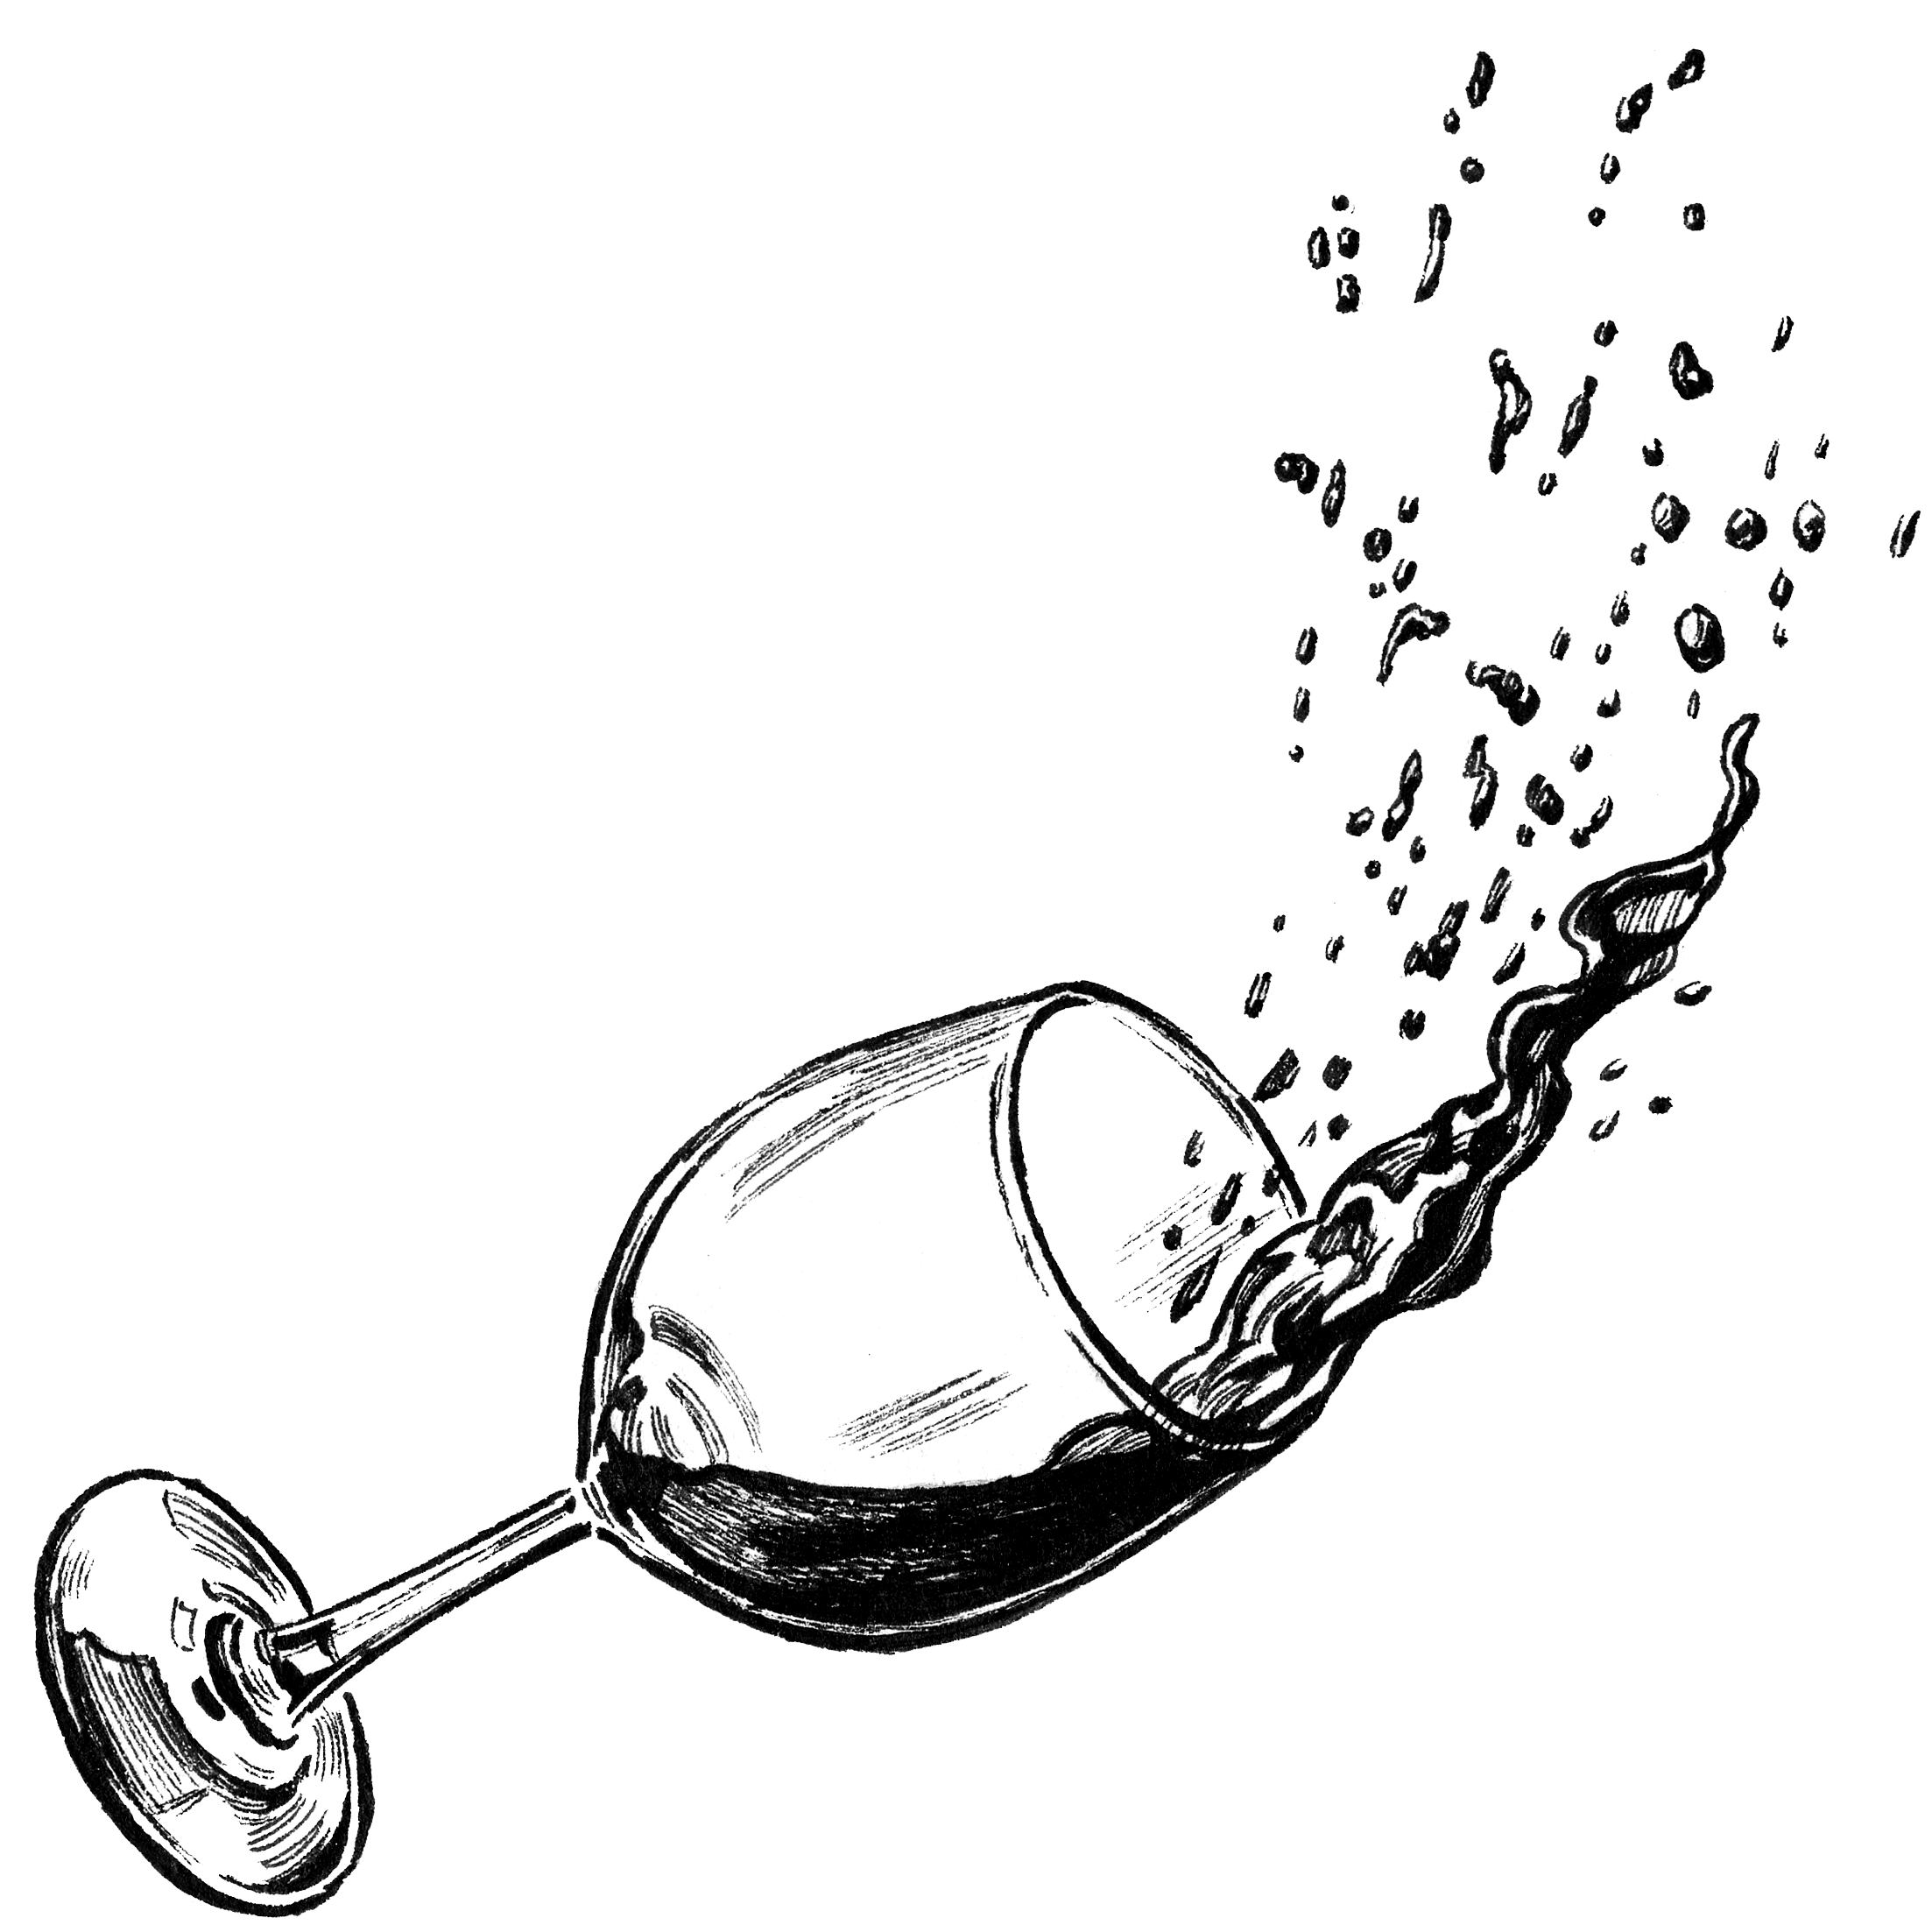
\includegraphics{wine.png}\end{textblock}
\begin{textblock}{1}(12.7,8.6)
\includegraphics[scale=.15]{stamp.png}\end{textblock}
\begin{tabular}{c||c}
\begin{tabular}{p{.45\textwidth}}
\multicolumn{1}{p{.45\textwidth}}{\centering\Huge\textsc{Aviation}}\\
   \large\centering 2 oz. Hendrick's, .5 oz. Luxardo Maraschino Liqueur, .5 oz. Creme de Violette, Fresh-Squeezed Lemon Juice. Garnished with a cherry.\\ 
\normalsize{Consider substituting with Creme Yvette.}\\
\makebox[.45\columnwidth]{\Huge\Dotfill}
\end{tabular}
\\
\begin{tabular}{p{.45\textwidth}}
\multicolumn{1}{p{.45\textwidth}}{\centering\Huge\textsc{Christmas Comes\\[-10pt]Only Once}}\\ 
   \large\centering 2 oz. Yamakazi 12 Year, 1 oz. Orgeat, .75 oz. Fresh-Squeezed Lemon Juice. Served over crushed ice.\\ 
\normalsize\textit{"No jokes, I've heard them all."}\\
\end{tabular}
&
\begin{tabular}{p{.45\textwidth}}
\multicolumn{1}{p{.45\textwidth}}{\centering\Huge\textsc{Earl Grey\\[-10pt]MarTEAni}}\\ 
   \large\centering 1.5 oz. Earl Grey Tanqueray, 1 oz. Simple Syrup, .5 oz. Fresh-Squeezed Lemon Juice, 1 Egg White. Garnished with a twist of lemon.\\
\normalsize\textit{"Every now and then a trigger has to be pulled..."}\\
\end{tabular}
\end{tabular}
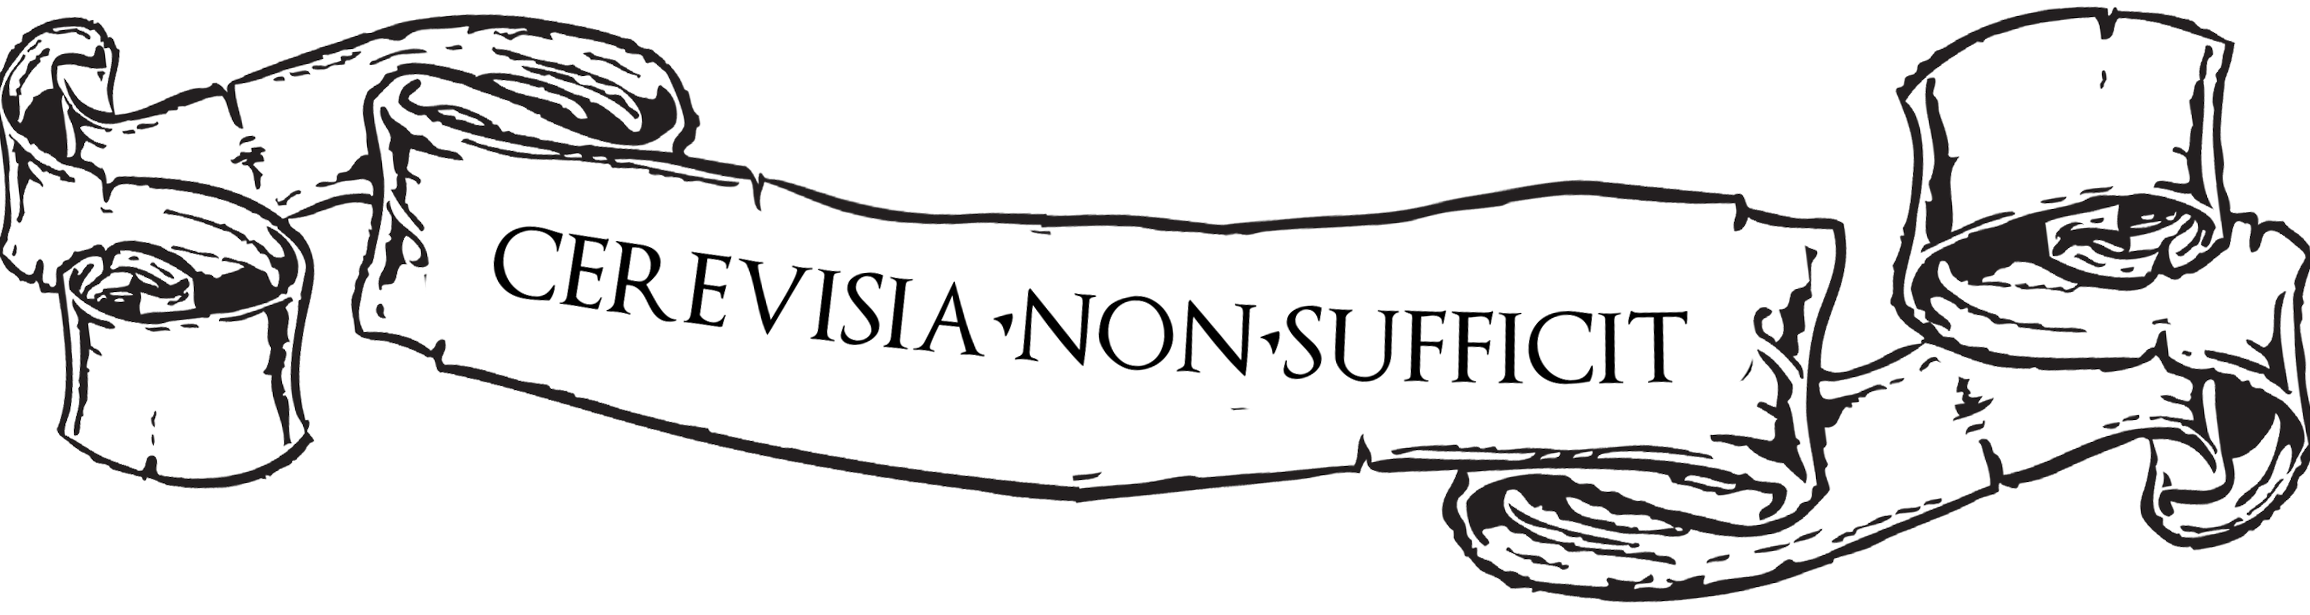
\includegraphics{logo.png}
\begin{tabular}{c||c}
\begin{tabular}{p{.45\textwidth}}
\multicolumn{1}{p{.45\textwidth}}{\centering\Huge\textsc{Eva Green}}\\ 
   \large\centering3 oz. Hendrick's, 1 oz. Grey Goose, .5 oz. Cocchi Americano, 1 Dash Lemon Bitters. Shake well until it is ice-cold then strain. Garnished with a twist of lemon.\\ 
\normalsize\textit{"Friend, bring me one as well. Hold the fruit."}\\\hfill
\end{tabular}
&
\begin{tabular}{p{.45\textwidth}}
\multicolumn{1}{p{.45\textwidth}}{\centering\Huge\textsc{Machete}}\\ 
   \large\centering2 oz. Jose Cuervo Blanco, 1 oz. Grand Marnier, 1 Fresh-Squeezed Lime, 1 Dash Tabasco Sauce. Garnished with a lime wedge. \\ 
\normalsize\textit{"You fucked with the wrong Mexican."}\\
\makebox[.45\columnwidth]{\Huge\Dotfill}
\end{tabular}
\\
\begin{tabular}{||p{.44\textwidth}||} \hline\hline
\\\centering\LARGE\textbf{``The problem with the world is that everyone is a few drinks behind.''\\ ...}\\ \Huge Humphrey Bogart
\end{tabular}
&
\begin{tabular}{p{.45\textwidth}}
\multicolumn{1}{p{.45\textwidth}}{{\vspace{-.3in}}\centering\Huge\textsc{New England,\\[-10pt]Old Fashioned}}\\ 
   \large\centering2 oz. Bacon Jack Daniels, .5 oz. Grade B Maple Syrup, 2 Dashes Angostura Bitters. Garnished with a candied orange peel. \\
\makebox[.45\columnwidth]{\Huge\Dotfill} 
\end{tabular}
\\
\begin{tabular}{p{.45\textwidth}} \hline\hline\\
\multicolumn{1}{p{.45\textwidth}}{\centering\Huge\textsc{Risico}}\\
   \large\centering1 oz. Rear Admiral Joseph, 1 oz. Gran Classico, 1 oz. Lillet Blanc. Garnished with a twist of grapefruit. \\
\normalsize\textit{"In this business there is much..."}\\
\end{tabular}
&
\begin{tabular}{p{.45\textwidth}}
\multicolumn{1}{p{.45\textwidth}}{\vspace{-.5in}\centering\Huge\textsc{Rehoboth Crush}}\\[-15pt] 
   \large\centering1.5 oz. Dogfish Head Blood Orange Vodka, 1 Fresh-Squeezed Orange, topped with Sprite. Garnished with a orange slice. \\
\normalsize\textit{"The Nectar of the Gods."}\\
\end{tabular}
\end{tabular}
\\[.25in]\makebox[\columnwidth]{\Huge\Dotfill}

\newpage %%%%%%%%%%%%
\customfont{
\makebox[\columnwidth]{\Huge\Dotfill}\\\centering\begin{spacing}{.4}{\Huge\color{BrickRed}\textbf{The Long List}}\end{spacing}
\makebox[\columnwidth]{\Huge\Dotfill}
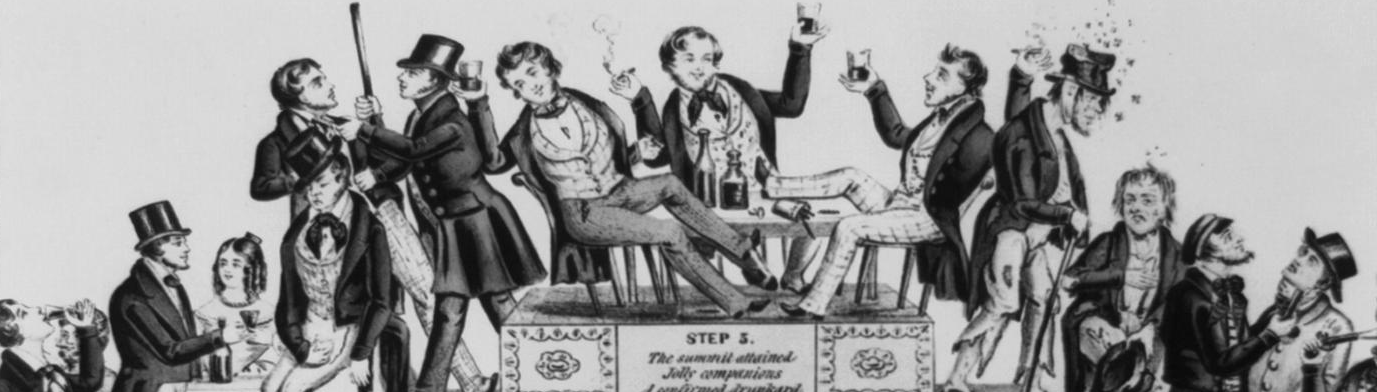
\includegraphics{longbanner.png}\\[-5pt]
\marginnote{\rotatebox{90}{
\begin{tabular}{l}
    \Huge\Dotfill \\
    \Huge Gin\hspace{6.7in} \\[-4pt]
    \Huge\Dotfill\\\vspace{-.35in}
\end{tabular}
}}
\begin{textblock}{1}(6.3,.6)\rotatebox{90}{\makebox[.56\paperheight]{\Huge\Dotfill}}\end{textblock}
\makebox[1.007\columnwidth]{\hspace{-.5in}\Huge\Dotfill}\\[-3pt]
{\small...ergo bibamus pro salute patriae.}\\[-5pt]
\makebox[\columnwidth]{\Huge\Dotfill}
\begin{tabular}{m{0.45\textwidth}m{0.05\textwidth}m{0.45\textwidth}}
{\centering\Huge{Albert Mathieu}\\*}
\centering 2 oz. Hendrick's, .75 oz. Lillet Blanc, .75 oz. Green Chartreuse, Splash of St. Germain, 1 Dash House Orange Bitters. Garnished with an orange twist. Stirred.\\
\centering\small{A marriage of British and French ingredients.}
&
&
{\centering\Huge{Bee's Knees}\\*}
\centering 2 oz. Tanqueray, .75 oz. Fresh-Squeezed Lemon Juice, .75 oz. Honey Syrup. Shaken.\\
\centering\small {"Bees? Beads!"}
\end{tabular}
\\\makebox[\columnwidth]{\Huge\Dotfill}

\begin{tabular}{m{0.45\textwidth}m{0.05\textwidth}m{0.45\textwidth}}
{\centering\Huge{Corpse Reviver\\[-10pt] No.400}\\*}
\centering .75 oz. Hendrick's, .75 oz. Grand Marnier, .75 oz. Cocchi Americano, .75 oz. Fresh-Squeezed Lemon Juice. Shaken.\\
\centering\small{OONS OONS OONS}
&
&
{\centering\Huge{Drax's Choice}\\*}
\centering1.5 oz. Tanqueray, .5 oz. Grand Marnier, .5 oz. Fresh-Squeezed Lime Juice, 2 Dashes Angostura Bitters. Stirred. \\
\centering\small{"I think he's attempting re-entry!"}
\end{tabular}
\\\makebox[\columnwidth]{\Huge\Dotfill}

\marginnote{\begin{sideways}\Huge Gin \end{sideways}}

\begin{tabular}{b{0.45\textwidth}m{0.05\textwidth}b{0.45\textwidth}}
{\centering\Huge{Evidence}\\*}
\centering 2 oz. Earl Grey Tanqueray, .5 oz. Lillet Blanc, .5 oz. Fresh-Squeezed Lemon Juice, 4 oz. Ginger Ale. Stirred. Garnished with a twist of lemon.\\
\centering\small{"...Or not pulled, it's hard to know which in your pajamas."}\\[-.3in]
\makebox[.49\columnwidth]{\hspace{-.1in}\Huge\Dotfill}
{\centering\Huge{French 150}\\*}
\centering 1 oz. Beefeater, .5 oz. Fresh-Squeezed Lemon Juice, .5 oz Simple Syrup. Shaken. Topped off with Boyer Brut and garnish with a twist of lemon. \\
\centering\small{"Twice as good as the French 75"}
&
&
{\hspace{-.225in}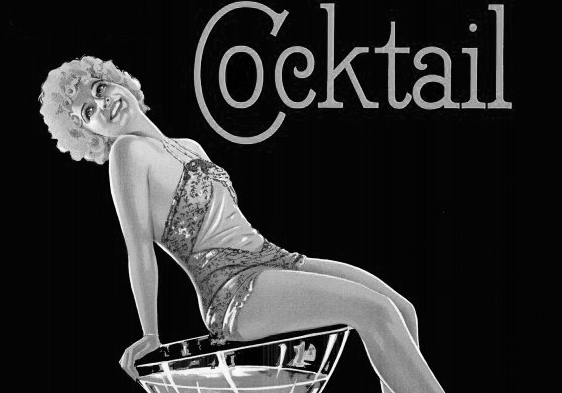
\includegraphics[scale=.85]{cocktail.png}}
\end{tabular}
\makebox[\columnwidth]{\Huge\Dotfill}

\begin{tabular}{m{0.45\textwidth}m{0.01\textwidth}m{0.465\textwidth}}
{\centering\Huge{Last Word}\\*}
\centering 1 oz. Hendrick's, 1 oz. Maraschino Liqueur, 1 oz. Green Chartreuse, 1 oz. Fresh-Squeezed Lime Juice. Shaken.\\
\centering\small{"Lawrence O'Donnell is an asshole."}
&
&
{\centering\Huge{Live and Let Cherry}\\*}
\centering 2 oz. Beefeater, 1 oz. Fresh-Squeezed Lemon Juice, .5 oz. Maraschino Liqeuer, .5 oz. Simple Syrup, 2 Muddled Cherries. Shaken. Served over crushed ice with a cherry.\\
\centering\small{When you've got a drink to make, you've gotta do it well.}
\end{tabular}
\makebox[\columnwidth]{\Huge\Dotfill}\\[-5pt]
{\Large\centering "I'm an advertising man, not a red herring. I've got a job, a secretary, a\\[-2pt] mother, two ex-wives and several bartenders dependent upon me and I\\[-2pt] don't intend to disappoint them by getting myself slightly killed!" \\[-2pt] \large Cary Grant in North By Northwest}\\[-2pt]
\makebox[1.007\columnwidth]{\hspace{-.5in}\Huge\Dotfill}\\[-1pt]
\marginnote{\rotatebox{90}{
\begin{tabular}{l}
    \Huge\Dotfill \\
    \Huge \hspace{1.4in} Brandy \hspace{7in} \\[-4pt]
    \Huge\Dotfill\\\vspace{-.35in}
\end{tabular}
}}
\makebox[1.007\columnwidth]{\hspace{-.5in}\Huge\Dotfill}\\
\begin{tabular}{m{0.45\textwidth}m{0.05\textwidth}m{0.425\textwidth}}
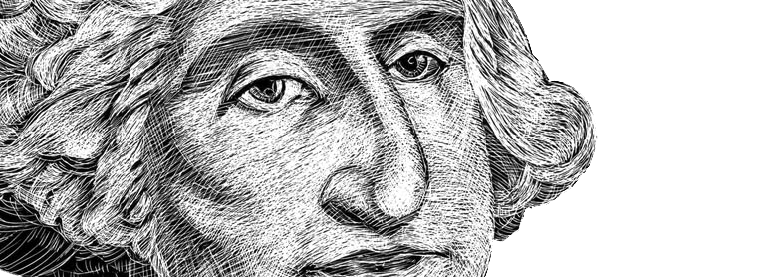
\includegraphics[scale=1]{patriot.png}
&
&
{\centering\Huge{Patriot}\\*}
\centering 1.5 oz. Beefeater, .5 oz. Fresh-Squeezed Lemon Juice, .75 oz. Simple Syrup. Club Soda, 4 Muddled Cherries, 8 Muddled Blueberries. Stirred. Topped with club soda. Garnished with a slice of lemon and cherry.\\
\centering\small{All hail Tom Brady.}
\end{tabular}\\[-4pt]
\makebox[\columnwidth]{\Huge\Dotfill}
\begin{textblock}{1}(6.3,0)\rotatebox{90}{\makebox[.23\paperheight]{\Huge\Dotfill}}\end{textblock}
\marginnote{\begin{sideways}\Huge Gin\end{sideways}}

\begin{tabular}{m{0.45\textwidth}m{0.05\textwidth}m{0.45\textwidth}}
{\centering\Huge{Pliny the Tonic}\\*}
\centering 2 oz. Hendrick's, .5 oz. Maraschino Liqueur, Cucumber, 1 Dash Peychaud's, 1 Dash Angostura. Muddle Cucumber with bitters. Stirred. Garnished with a slice of cucumber.\\
\centering\small{ex Africa semper aliquid novi.}
&
&
{\centering\Huge{Strawberry Fields}\\*}
\centering 2 oz. Plymouth, .5 oz. St. Germain, .5 oz. Simple Syrup, Two Strawberries, Fresh-Squeezed Lime Juice. Shake of Basil and Parsley. Stirred.\\
\centering\small{"I can't find the... um... the stationery."}
\end{tabular}
\\\makebox[\columnwidth]{\Huge\Dotfill}

\begin{tabular}{m{0.45\textwidth}m{0.05\textwidth}m{0.45\textwidth}}
{\centering\Huge{Vieux Mot}\\*}
\centering 1.5 oz. Hendrick's, .75 oz. Fresh-Squeezed Lemon Juice, .5 oz. St. Germain, .5 oz. Simple Syrup. Shaken. Garnished with a cherry.\\
\centering\small{Old Word}
&
&
{\centering\Huge{White Lady}\\*}
\centering 2 oz. Tanqueray, .75 oz. Cointreau, .75 oz. Fresh-Squeezed Lemon Juice, 1 Egg White. Shaken.\\
\centering\small{Consider alternating Laird's Bonded for a Pink Lady.}
\end{tabular}
\makebox[\columnwidth]{\Huge\Dotfill}\\[-3pt]
{\small "Ready your breakfasts and eat hearty, for tonight we drink in hell!" - Leonidas of Sparta}\\[-5pt]
\makebox[\columnwidth]{\Huge\Dotfill}\\
\begin{textblock}{1}(6.3,0.1)\rotatebox{90}{\makebox[.24\paperheight]{\Huge\Dotfill}}\end{textblock}
\begin{tabular}{m{0.45\textwidth}m{0.01\textwidth}m{0.45\textwidth}}
{\centering\Huge{Applejack Rabbit}\\*}
\centering 2 oz. Laird's, .75 oz. Fresh-Squeezed Lemon Juice, 1 Fresh-Squeezed Orange, .5 oz. Grade B Maple Syrup, Shaken.\\
\makebox[.48\columnwidth]{\hspace{-.2in}\Huge\Dotfill}\\
{\centering\Huge{Face Like a Pig}\\*}
\centering 2 oz. Nigori Sake, 1 oz. Cognac, 1 tablespoon Vanilla Extract, 3 dashes Whiskey-Aged Bitters. Stirred. Garnished with grated nutmeg.\\
\centering\small{You only live twice\\Once when you're born\\And once when you look death in the face}
&
&
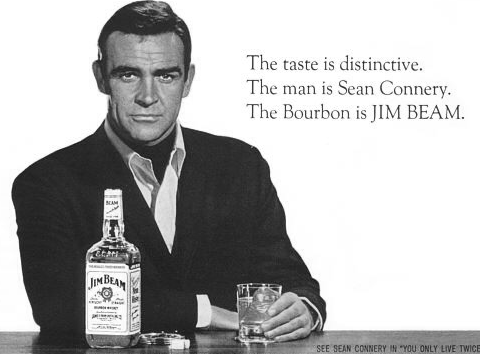
\includegraphics[scale=.68]{connery.png}
\end{tabular}
\\\makebox[\columnwidth]{\Huge\Dotfill}
\begin{textblock}{1}(6.3,0)\rotatebox{90}{\makebox[.25\paperheight]{\Huge\Dotfill}}\end{textblock}
\begin{tabular}{m{0.45\textwidth}m{0.05\textwidth}m{0.45\textwidth}}
{\centering\Huge{Great Punkin'}\\*}
\centering 2 oz. Dogfish Head Punkin' Ale, 1 oz. Bulleit, 1 oz. Laird's, .5 oz. Grade B Maple Syrup, 1 Egg. Add everything to mixing glass and swirl beer. Shakened. Garnished with nutmeg.\\
\centering\small{"Winter is Coming, Charlie Brown!"}
&
&
{\centering\Huge{Putting on the Ritz}\\*}
\centering 1 oz. Cognac, .5 oz. Triple Sec, 2 tablespoons Maraschino Liqueur, .5 oz. Fresh-Squeezed Lemon Juice, Boyer Brut. Stirred. Topped off with Boyer Brut. Garnished with an orange twist.\\
\centering\small{"If you're blue and you don't know where to go to..."}
\end{tabular}
\\\makebox[\columnwidth]{\Huge\Dotfill}

\marginnote{\begin{sideways}\Huge \end{sideways}}

\begin{tabular}{m{0.45\textwidth}m{0.05\textwidth}m{0.45\textwidth}}
{\centering\Huge\textsc{Sidecar}\\*}
\centering 2 oz. Cognac, .75 oz. Cointreau, .75 oz.  Fresh-Squeezed Lemon Juice, .25 oz. Simple Syrup. Shaken. Served with lemon-moistened, lightly sugar-coated rim.\\
&
&
{\centering\Huge\textsc{Vanilla Punch}\\*}
\centering 2 oz. Brandy, 2 teaspoons Sugar, .5 oz. Fresh-Squeezed Lemon Juice, Vanilla extract (to taste).. Shaken. Served over crushed ice and garnished with a slice of lemon.\\
\end{tabular}
\makebox[1.007\columnwidth]{\hspace{-.5in}\Huge\Dotfill}\\[-3pt]
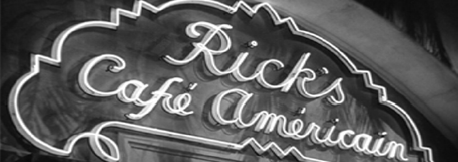
\includegraphics[scale=1.5]{americain.png}
\marginnote{\rotatebox{90}{
\begin{tabular}{l}
    \Huge\Dotfill \\
    \Huge \hspace{2.7in} Whisk(e)y \hspace{2.7in} \\[-4pt]
    \Huge\Dotfill\\\vspace{-.35in}
\end{tabular}
}}
\makebox[1.007\columnwidth]{\hspace{-.5in}\Huge\Dotfill}\\[-3pt]
\begin{textblock}{1}(6.3,0)\rotatebox{90}{\makebox[.395\paperheight]{\Huge\Dotfill}}\end{textblock}
\begin{tabular}{m{0.45\textwidth}m{0.05\textwidth}m{0.45\textwidth}}
{\centering\Huge\textsc{Alpoe}\\*}
\centering 2 oz. Four Roses, .75 oz. Fresh-Squeezed Lemon Juice, .5 oz. Grade B Maple Syrup, .25 oz.  Maraschino Liqueur, 1 Dash Orange Bitters, Habanero Bitters soaked Sugar Cube. Shaken. Garnished with an orange twist.\\
\centering\small{"Go. For it."}
&
&
{\centering\Huge\textsc{Grade B\\[-10pt] Maple Leaf}\\*}
\centering 2 oz. Jack Daniels, .75 oz. Grade B Maple Syrup, .75 oz. Fresh-Squeezed Lemon Juice. Shaken.  Garnished with a cinnamon stick.\\
\centering\small{"As of course is tradition."}
\end{tabular}
\\\makebox[\columnwidth]{\Huge\Dotfill}
\begin{tabular}{m{0.45\textwidth}m{0.05\textwidth}m{0.45\textwidth}}
{\centering\Huge{Manhattan}\\*}
\centering 2 oz. Bulleit, 1 oz. Cocchi Americano, 1 Dash Angostura Bitters, 1 Dash Whiskey Barrel-Aged Bitters. Stirred. Garnished with a cherry.\\
\centering\small{A fresh take on the old classic.}\\
&
&
{\centering\Huge\textsc{Not Half Bad}\\*}
\centering 2 oz. Rittenhouse, 1 oz. Maraschino Liqeuer, .5 oz. Simple Syrup, 2 Dashes Angostura Bitters. Shaken. \\
\centering\small{"I ought to think up a name for this..."}
\end{tabular}\\[-4pt]
\makebox[\columnwidth]{\Huge\Dotfill}

\begin{tabular}{m{0.45\textwidth}m{0.05\textwidth}m{0.46\textwidth}}
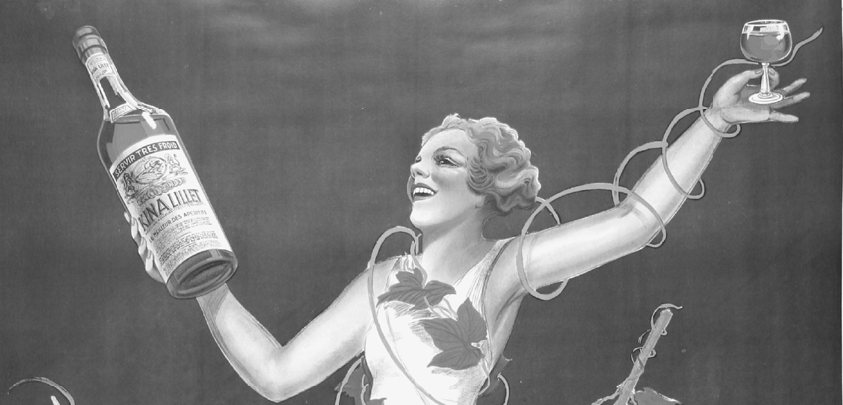
\includegraphics[scale=.39]{kina.png}
&
&
{\centering\Huge\textsc{That's Why They\\[-10pt] Call Me Whiskey}\\*}
\centering 1 oz. Jack Daniel's, .5 oz. Cointreau, 3 Dashes Peychaud's Bitters, 2 Dashes Angostura Bitters. Stirred. Topped with Brut and garnished with an orange twist.\\
\centering\small{For those as curious as a cat.}
\end{tabular}
\makebox[\columnwidth]{\Huge\Dotfill}\\[-3pt]
{\small "Always do sober what you said you'd do drunk. That will teach you to keep your mouth shut." - Ernest Hemmingway}\\[-5pt]
\makebox[\columnwidth]{\Huge\Dotfill}\\
\begin{textblock}{1}(6.3,0)\rotatebox{90}{\makebox[.25\paperheight]{\Huge\Dotfill}}\end{textblock}
\begin{tabular}{m{0.45\textwidth}m{0.05\textwidth}m{0.45\textwidth}}
{\centering\Huge\textsc{The Saugerties}\\*}
\centering 1.5 oz. Rye, .75 oz. Dry Vermouth, .5 oz. Fresh-Squeezed Lemon Juice, .5 oz. Simple Syrup, 3 Dashes Orange Bitters, 1 Egg White. Shaken. Garnished with a cherry.\\
&
&
{\centering\Huge\textsc{Triple Crown and\\[-10pt] Travers Too}\\*}
\centering 1.25 oz. Jack Daniels, .75 oz. Cognac, .5 oz. Simple Syrup, 12 Muddled Mint Leaves. Topped with layers of cracked ice and mint, then frozen.\\
\centering\small{"Daddy Nose Best"}
\end{tabular}
\\\makebox[\columnwidth]{\Huge\Dotfill}

\begin{tabular}{m{0.45\textwidth}m{0.05\textwidth}m{0.45\textwidth}}
{\centering\Huge\textsc{The Stamford}\\*}
\centering 1.5 oz. Bulleit, .5 oz. Laird's Bonded, .75 oz.  Fresh-Squeezed Lemon Juice, .75 oz Orgeat, 4-5 Dashes Angostura Bitters. Shaken, then Stirred over crushed ice. Topped with bitters and garnished with grated cinnamon.
&
&
{\centering\Huge\textsc{Yamakazi\\[-10pt]SMASH!!!}\\*}
\centering 2 oz. Yamakazi 12 Year, 3 Lemon Wedges, .75 oz.  Simple Syrup, 6 Muddled Mint Leaves. Shaken. Garnished with mint.\\
\end{tabular}
\\\makebox[1.007\columnwidth]{\hspace{-.5in}\Huge\Dotfill}\\[-3pt]
\marginnote{\rotatebox{90}{
\begin{tabular}{l}
    \Huge\Dotfill \\
    \Huge\hspace{.32in} Tequila, Rum, etc. \hspace{.5in} \\[-4pt]
    \Huge\Dotfill\\\vspace{-.35in}
\end{tabular}
}}
\makebox[1.007\columnwidth]{\hspace{-.5in}\Huge\Dotfill}\\[-3pt]
{\small "So we beat on, boats against the current, borne back ceaselessly into the past." - F. Scott Fitzgerald}\\[-5pt]
\makebox[\columnwidth]{\Huge\Dotfill}\\[-3pt]
\begin{textblock}{1}(6.3,0)\rotatebox{90}{\makebox[.35\paperheight]{\Huge\Dotfill}}\end{textblock}
\begin{tabular}{m{0.45\textwidth}m{0.05\textwidth}m{0.45\textwidth}}
{\centering\Huge\textsc{El Burro del Diablo}\\*}
\centering 1.5 oz. Jose Silver, .75 oz. Creme de Cassis, .75 oz. Fresh-Squeezed Lime Juice, Ginger Ale. Shaken. Topped with ginger ale/beer and garnished with a lime wheel.\\
\centering\small{The other mule never made it from Moscow.}
&
&
{\centering\Huge\textsc{Tequila Smash}\\*}
\centering 2 oz. Jose Silver, .5 oz. Maraschino Liqueur, .5 oz. Fresh-Squeezed Lime Juice, 4 Muddled Cherries, 4 Muddled Blueberries. Shaken.  Garnished with a skewered blueberry, lime wheel and cherry.
\end{tabular}
\\\makebox[\columnwidth]{\Huge\Dotfill}

\begin{tabular}{m{0.45\textwidth}m{0.05\textwidth}m{0.45\textwidth}}
{\centering\Huge\textsc{Lovely St. Rita}\\*}
\centering 2 oz. Jose Silver, 1 oz. St. Germain, 1 Fresh-Squeezed Lime. Shaken.  Garnished with lime wedge.\\
\centering\small{"Looks like a Rita to me."}
&
&
{\centering\Huge\textsc{Airmail}\\*}
\centering 2 oz. Bacardi, .5 oz. Fresh-Squeezed Lime Juice, .5 oz. Honey Syrup, 1 oz. Boyer Brut. Shaken. Topped with Boyer Brut and garnished with a lime wheel.\\
\centering\small{“It ought to make you fly high.”}
\end{tabular}
\\\makebox[\columnwidth]{\Huge\Dotfill}

\begin{tabular}{m{0.45\textwidth}m{0.05\textwidth}m{0.45\textwidth}}
{\centering\Huge\textsc{Please Don't Tell\\[-10pt] Paddington}\\*}
\centering 1.5 oz. Bacardi, .5 oz. Lillet Blanc, .5 oz. Fresh-Squeezed Grapefruit, .5 oz. Fresh-Squeezed Lemon Juice, 1 teaspoon Orange Marmalade. Shaken. Garnished with a twist of grapefruit.
&
&
{\centering\Huge\textsc{The Saratoga}\\*}
\centering 3 oz. fruit-infused Shiraz, 1 oz. Three Olives Raspberry, 1 oz. Bacardi Limon, Splash of Sour Mix, Splash of Sprite. Garnished with soaked fruit.\\
\centering\small{Sangria at its finest.}
\end{tabular}
\\\makebox[1.007\columnwidth]{\hspace{-.5in}\Huge\Dotfill}\\[-.2in]
\marginnote{\rotatebox{90}{
\begin{tabular}{l}
    \Huge\Dotfill \\
    \Huge\hspace{.8in}Multiple Choice\hspace{.8in} \\[-4pt]
    \Huge\Dotfill\\\vspace{-.35in}
\end{tabular}
}}
\begin{tabular}{m{0.45\textwidth}m{0.05\textwidth}m{0.45\textwidth}}
\\\centering\large Balance \& structure are the hallmarks of a classically constructed cocktail. I provide those\textemdash you choose the base spirit.
\\[.2in]{\Large St. Germain and \\ Champagne with:}\\\normalsize a. Hendrick's Gin\\b. Dogfish Head Darkside Rum\\c. Jose Cuervo Silver Tequila\\d. Cognac
\\[.3in]{\Large Cocchi Americano, Fresh-Squeezed Lemon Juice, and Angostura Bitters with:}\\{\normalsize a. Beefeater Gin\\b. Bulleit Rye\\c. Laird's Applejack\\d. Cognac}
&
&
\centering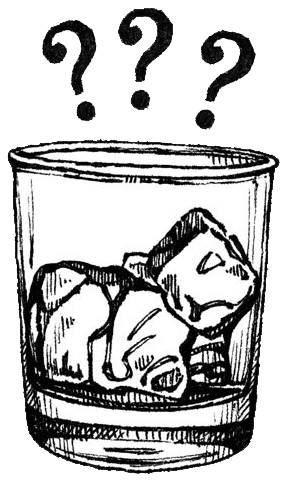
\includegraphics[scale=.48]{multichoice.png}\\
{\Large Luxardo Maraschino Liqueur, Fresh-Squeezed Lemon Juice, and Fruit over crushed ice with:}\normalsize \\a. Plymouth Gin\\b. Dogfish Head Darkside Rum\\c. Jose Cuervo Silver Tequila\\ d. Laird's Applejack
\end{tabular}
\makebox[\columnwidth]{\Huge\Dotfill}\\[-3pt]
{\small "I hate small portions of anything, particularly when they taste bad." - Ian Fleming}\\[-5pt]
\marginnote{\rotatebox{90}{
\begin{tabular}{l}
    \Huge\Dotfill \\
    \Huge\hspace{.00in}Barstock \hspace{.00in} \\[-4pt]
    \Huge\Dotfill\\\vspace{-.35in}
\end{tabular}
}}
\makebox[1.007\columnwidth]{\hspace{-.5in}\Huge\Dotfill}\\
}
{\begin{spacing}{.1}\scriptsize\raggedright\textbf{Fruit:} Lemon, Lime, Orange \textbf{Garnishes:} Whiskied Cherries, Citrus Twists, Fresh Mint, Cucumber (peel first, slice into wheels), Fresh, Large Organic Eggs, Maple Syrup (Grade B) \textbf{Carbonated Beverages:} Tonic Water, Q Club, Q Ginger, Champagne (Boyer Brut), Sprite, Cola \textbf{Spices/Sweetener:} Nutmeg, Simple Syrup, Honey Syrup, Orgeat, Salt, Cinnamon \textbf{Vodka:} Grey Goose, Skyy, Dogfish Head Blood Orange, Absolut Raspberry, Kichom Nikaido \textbf{Gin:} Beefeater, Tanqueray, Hendrick's, Tanqueray (Earl-Grey infusion) \textbf{Rum:} Bacardi, Gosling's Black Seal, Dogfish Head Dark Side Rum, Dogfish Head White Light Rum (Banana+Brown Sugar Infusion)  \textbf{Cognac/Brandy:} Hine V.S.O.P., Laird's Bonded Apple Brandy, Laird's Applejack \textbf{Tequila:} Jose Cuervo Silver, Sombra \textbf{Whisk(e)y/Rye:} Four Roses, Jack Daniels, Gentleman Jack, Maker's Mark, Jack Daniels (Bacon infusion), Yamakazi 12 yr., Bulleit Rye, Jameson, Famous Grouse \textbf{Herbal/Floral:} Green Chartreuse, Yellow Chartreuse, Creme de Violette, Creme Yvette, St. Germain, Clear Creek Douglas Fir \textbf{Peel/Fruit:} Cointreau, Grand Marnier, Luxardo Maraschino, Triple Sec \textbf{Nut/Bean/Seed:} Kahlua, Creme de Cacao, Vanilla Liqueur (optional) \textbf{Apertifs/Vermouths:} Cocchi Americano, Lillet Blanc, Campari, Dry+Sweet Vermouths \textbf{Bitters:} Angostura, Fee Brothers Old Fashioned Aromatic Bitters, Fee Brothers Lemon Bitters, Fee Brothers West Indian Orange Bitters, Fee Brothers Whiskey-Barrel Aged Old Fashioned Aromatic Bitters, Fee Brothers Cherry Bitters, Peychaud's Bitters, Regan's Orange Bitters No. 6, Bitter Truth Jerry House Decanter Bitters, Bitter Truth Celery Bitters, Bar Keep Lavender Bitters, Bittermen's Boston Bittahs, Bitterman's Habanero Shrub Bitters, Dr. Adam Elmegirab's Boker Bitters, Dr. Adam Elmegirab's Aphrodite Bitters, Dr. Adam Elmegirab's Christmas Bitters, House Orange Bitters (1:1 Fee Brothers' Orange and Regan's Orange) \textbf{Beer:} Dogfish Head 120 Minute IPA, Dogfish Head World Wide Stout, Dogfish Head Festina Peche, Dogfish Head Punkin' Ale, Dogfish Head Rhizing Bines, Yebisu, Sapporo, Guinness\\\hfill\end{spacing}}
\customfont{\makebox[1.007\columnwidth]{\hspace{-.5in}\Huge\Dotfill}}

\end{document}

%%%%%%%%%
ON QUEUE
%%%%%%%%%
Barstock:


creme de cacao, dry vermouth, lemon juice
a. gin
b. rye
c. rum
d. vodka (with grenadine)

CHARMING SNAKE: Kentucky Straight Bourbon, Garam Masala, Habanero Bitters (rocks)
Sunset at Gowanus: Rum, Laird's Applejack, Yellow Chartreuse, Fresh Lime Juice, Maple Syrup
Peter's Word: Laphroaig Single Malt Scotch, Luxardo Maraschino Liqueur, Green Chartreuse, Fresh Lime Juice
Fancy Holland Royale: Champagne, Bols Genever Gin, Grand Marnier, Dash of Fee’s Barrel Aged Bitters
Dark N Bubbly: Champagne, Goslings Rum, Ginger Syrup, Fresh Lime Juice
Tailspin: Beefeater Gin, Carpano Antica Vermouth, Green Chartreuse, Campari, House Orange Bitters, Garnished with a Lemon Twist
Bourbon Sour: Bourbon, Lemon, Egg White, Angostura Bitters
Corpse Reviver No. 1: Applejack, Sweet Vermouth, Brandy
El Floridita No. 1: Rum, Maraschino Liqeur, Lime, Simple Syrup
Saratoga Cocktail: 1:1:1 brandy, rye, sweet vermouth, angostura
mai tai: 2:2:1:1 dark, light rum, grand marnier, lime juice, orgeat
Seelbach Cocktail: 1oz Bourbon, .5 triple sec, 7 dashes angostura+peychaud's, top off with brut orange twist

Sour/Short
Crescent City: Jamaican Rum, Sweet Vermouth, Lime, Angostura Bitters
Royal Bermuda Yacht Club Cocktail: Nicaraguan Rum, Lime, Falernum, Curacao
Southside: Plymouth Gin, Lime, Mint
Davis Cocktail: Dry Vermouth, Jamaican Rum, Lemon, Grenadine

Herbal/Spirituous
Astoria: Tom Gin, Dry Vermouth, Orange Bitters
Martinez: Genever, Sweet Vermouth, Maraschino, Bokers Bitters
Cotton Cocktail: Rye, Sweet & Dry Vermouth, Orange Bitters
Sazerac: Rye, Turbinado, Absinthe, Angostura & Peychaud’s Bitters
Tipperary: Irish Whisky, Sweet Vermouth, Green Chartreuse
Gin Daisy: Tom Gin, Lemon, Yellow Chartreuse, Orange Bitters
Vieux Carre: Rye, Cognac, Sweet Vermouth, Benedictine, Angostura & Peychaud’s Bitters
Champs-Elysees: Cognac, Green Chartreuse, Lemon, Simple Syrup, Angostura. 
Harvest Moon: Rye, Lillet Blanc, Laird's, Green Chartreuse, Orange Bitters
Tuxedo: Dry Gin, Dry Vermouth, Maraschino, Absinthe

Boozy/Alluring
Old-Fashioned: Bourbon, Sugar Cube, Angostura Bitters
Fourth Regiment: Rye, Sweet Vermouth, Orange, Peychaud's & Celery Bitters
Corn N’ Oil: Dark Virgin Islands Rum, Falernum, Angostura Bitters
Improved Holland Gin Cocktail: Genever, Maraschino, Turbinado, Peychaud's & Angostura Bitters
Japanese: Cognac, Orgeat, Angostura
Creole Contentment: Cognac, Madeira, Maraschino, Orange Bitters

Light/Long
Long Island Tea: Tom Gin, Blanco Tequila, Agricole Rhum, Lemon, Triple Sec, Vodka
Rubus Swizzle: Nicaraguan Rum, Lemon, Raspberry, Orgeat
Mexican Firing Squad Special: Blanco Tequila, Lime, Grenadine, Angostura Bitters
Black \& Tan: Rye, Lime, Blackberries, Mint, Ginger Beer
Bramble: Dry Gin, Lemon, Crème de Cassis
Rye Buck: Rye, Ginger Beer
Gin \& Tonic: Dry Gin, Tonic Water
Tequila Sunrise: Blanco Tequila, Lemon, Crème de Cassis, Grenadine
Hemingway Daiquiri: Panamanian White Rum, Lime, Grapefruit, Maraschino
Daisy de Santiago: Panamanian White Rum, Lime, Yellow Chartreuse, Soda
The Ramos Fizz: 1.5 oz Plymouth, 1 oz heavy cream, 1 egg white, .75 oz simple syrup, .5 oz fresh lime juice, .5 oz fresh lemon juice, .75 tsp orange flower water, 1 oz sparkling water